\documentclass{mipt-thesis-bs}
\usepackage{mipt-thesis-biblatex}

\addbibresource{main.bib}

\title{Система мененджмента аккумуляторных батарей с активной балансировкой ячеек: современные проблемы, пути совершенствования, применение в авиастроении.}
\author{Бортник С.\,М.}
\supervisor{Киселёв И.\,С.}
\studyprofile{Выпускная квалификационная работа бакалавра по направлению 09.03.01}
\studyprofilename{<<Информатика и вычислительная техника>>}
\groupnum{Б03-115У}
\faculty{Факультет аэродинамики и летательной техники}
\department{Кафедра силовых установок ЦИАМ}

\DeclareAcronym{bms}{
  short=BMS,
  long=Battery Managment System,
}

\DeclareAcronym{soc}{
  short=SOC,
  long=State of Charge,
}

\DeclareAcronym{su}{
  short=СУ,
  long=cиловые установки,
}

\begin{document}


\section{TO DO LIST}

\begin{itemize}
    \item [*] Ссылки для оглавления
    \item [*] Написать введение (ПОСЛЕ НАПИСАНИЯ ОБЗОРА)
\end{itemize}

\frontmatter
\titlecontents

\chapter{Сокращения}
\printacronyms[heading=none]

\mainmatter

\chapter{Введение}


% \begin{figure}[h]
% 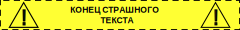
\includegraphics[width=\linewidth]{img/warning.png}
% % \caption{A boat.}
% % \label{fig:boat1}
% \end{figure}
% Figure \ref{fig:boat1} shows a boat.

% \warningbeg % ПРАВИТЬ!
Введение нужно написать в самом конце. \\
Пока что тут будет просто план:        \\
- Что то про развитие (электромобили, беплы)  \\
- Про необходимость балансировки  \\
- Что нибудь ещё \\
Для справки
% Собснаа все по госту(нет)
\begin{figure}[h]
    \fbox{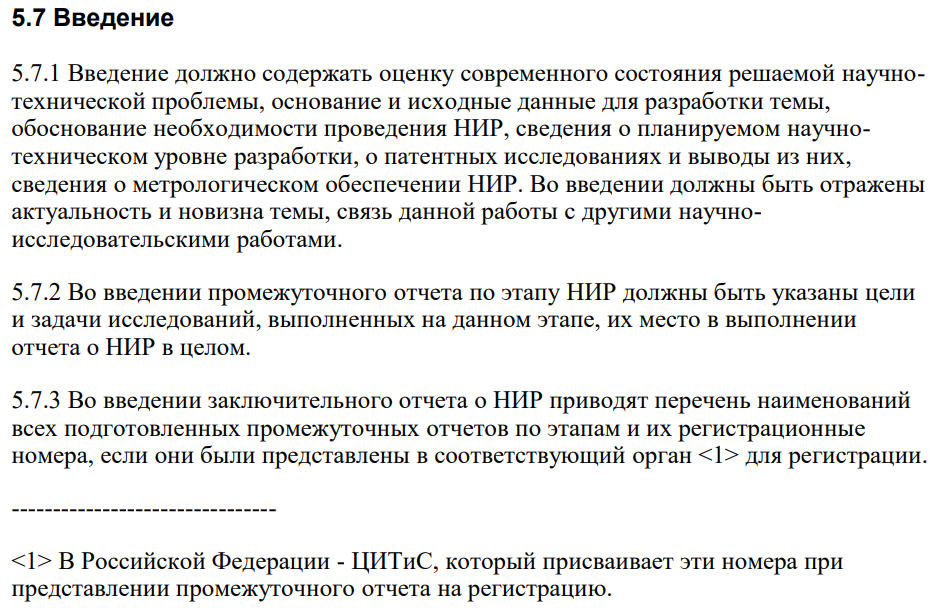
\includegraphics[width=420px]{img/dev/GOST_intro.png}}
\end{figure}

% \warningend % ПРАВИТЬ!
\newpage

% За последние 20 лет появилось огромное количество
% На сегодняшний день известно множевство различных аккумуляторных элементов

% К сожалению электродвигатели уступают по удельной мощности жидкостнотопливным реактивным и поршневым \aca{su}. 
% В качестве примера подойдёт проект NASA X-57 ''Maxwell''

% Rotax 912S3 
% Мощность:  2 × 100 л.с..
% Резюмируя вышесказанное - наиболее используемые литий-полимерные аккумуляторы сильно уступают существующим \aca{su}.
% Однако не стоит недооценивать важность \aca{bms} для авиастроениия. Подобную систему контроля можно использовать и с другими типами ... , например суперкондестаторы
% Возможно в будущем будут открыты 'тёплые' сверхпроводники, что позволит увеличить удельную мощность электродвигателей в n раз (см. Источник)  
% По этому данный материал стоит рассматривать не более чем научно-технический задел



\chapter{Технический обзор}
\section{Литий-ионные батареи -- обзор}
% За последние десятилетия литий-ионные аккумуляторы превратились из дорогих и не распространённых 
% в стандартные источники питания, используемые в самых различных областях. 
% Стоит сразу отметить, что для литий-ионного аккумулятора характерна высокая пожароопасность, об этом будет сказано ниже. \\
% Несмотря на то технология литиевых источников тока была известна достаточно давно, 
% и в конце XX века литиевые батареи активно использовались в различных устройствах.
% Только в 1991 году Акира Ёсино изобрёл литий-ионный аккумулятор, который широко используется сегодня. 
% Данная технология позволила значительно увеличить плотность энергии. (см. статью\cite{admt_201700376} ). 

% Как бы хорошо не был «укрощен» литий, аккумулятор остаётся опасным устройством, 
% так как в его составе находятся сильный окислитель и восстановитель, разделённые тонким полимерным сепаратором. 
% При нарушении целостности сепаратора происходит каскадная реакция, сопровождаемая нагревом.
% Содержимое аккумулятора превращается в первокласную взрывчатую смесь топлива и окислителя. И эту субстанцию уже подожгли.
% Существует много встроенных мер обеспечения безопасности Li-ion аккумуляторов, которые работают автономно.
% Но литий-ионные аккумуляторы остаются достаточно чуствительными к небрежной эксплуатации. 
% Там, где применяется литий-ионный аккумулятор, нет места простейшим зарядным устройствам из мира «свинца» и «никель-кадмия». 
% Зарядное устройство обязано быть «умным». Процесс зарядки литий-ионного аккумулятора многостадийный, 
% предполагает строгое выдерживание параметров, должен быть вовремя завершен. Перекладывание ответственности на пользователя не допустимо.

% Основными проблемами эксплуатации можно назвать перезаряд и переразряд.
% Иначе можно сказать, что важно выдерживать оптимальный диапазон напряжений при работе с аккумулятором.
% Перенапряжение в ячейке приводит к электролизу компонентов электролита и дальнейшему выделению газов, 
% давление которых может нарушить герметичность аккумулятора, 
% это также приводит к пожару так как получившая смесь графита и лития самовоспламеняется на воздухе.
% При больших токах разряда(графит не успевает «впитывать» литий) 
% и при переразряде(графит теряет активную поверхность) образуется металлическая фаза лития, 
% которая в дальнейшем приводит к образованию дендритов(древовидные образования) нарушающих обшивку аккумулятора. 
% Опасна и перегрузка во время разряда. 
% Перегрев вызывает вскипание или термическое разложение электролита, 
% выделение кислорода из катодной активной массы, повреждение сепаратора. В результате -- короткое замыкание и взрыв. 
% Подобные результат будет при повреждении ячейки, только к окислителю добавится кислород из атмосферы.




% В последние десятилетия литий-ионные аккумуляторы прошли путь от дорогостоящей и малораспространённой технологии 
% до универсального источника питания, применяемого в самых разнообразных сферах.

% Стоит отметить, что одним из ключевых недостатков литий-ионных батарей является их высокая пожароопасность, 
% что подробно рассмотрено далее.

% Хотя принципы работы литиевых источников тока были известны уже давно, 
% лишь к концу XX века литиевые батареи начали активно использоваться в электронике. 
% Прорыв в этой области произошёл в 1991 году, когда Акира Ёсино разработал литий-ионный аккумулятор, 
% ставший основой для современных энергоносителей. 
% Внедрение этой технологии позволило существенно увеличить плотность хранения энергии (см. статью \cite{admt_201700376}).

% Несмотря на успешное решение многих технических проблем, литий-ионные аккумуляторы остаются потенциально опасными устройствами. 
% Это обусловлено тем, что в их конструкции содержатся мощные окислитель и восстановитель, разделённые тонким полимерным сепаратором. 
% Если его целостность нарушается, запускается каскадная реакция, сопровождающаяся интенсивным нагревом. 
% В результате содержимое аккумулятора превращается в высокоэнергетическую смесь топлива и окислителя, готовую к воспламенению.

% Для снижения рисков в конструкции Li-ion батарей предусмотрено множество автономных систем безопасности. 
% Однако, несмотря на эти меры предосторожности, аккумуляторы остаются весьма чувствительными к неправильной эксплуатации. 
% Они требуют использования специализированных зарядных устройств, 
% поскольку применение примитивных аналогов, разработанных для свинцово-кислотных или никель-кадмиевых батарей, 
% может привести к катастрофическим последствиям. Процесс зарядки литий-ионных элементов многостадийный и требует точного 
% соблюдения параметров, исключая возможность случайных ошибок со стороны пользователя.

% К числу основных эксплуатационных проблем можно отнести перезаряд и переразряд. 
% Оптимальный диапазон напряжений должен строго выдерживаться при работе с аккумулятором. 
% Перенапряжение внутри ячейки способно вызвать электролиз компонентов электролита с последующим выделением газов, 
% что может привести к разгерметизации батареи и возникновению пожара. Это обусловлено тем, что смесь лития и графита, 
% оказавшись в контакте с воздухом, самовоспламеняется.

% Высокие токи разряда или глубокий переразряд также представляют серьёзную угрозу. 
% В первом случае графитовая структура не успевает поглощать литий, 
% а во втором теряет активную поверхность, что способствует образованию металлической фазы лития. 
% Со временем это может привести к росту дендритов — иглообразных кристаллов, разрушающих оболочку аккумулятора.

% Не менее опасна перегрузка во время разряда. Перегрев приводит к закипанию или термическому разложению электролита, 
% выделению кислорода из катодного материала и разрушению сепаратора. 
% Всё это ведёт к короткому замыканию и возможному взрыву. 
% Если же повреждение ячейки сопровождается попаданием кислорода из окружающей среды, 
% вероятность возгорания возрастает многократно.
















% Перегрев вызывает вскипание или термическое разложение электролита, 
% выделение кислорода из катодной активной массы, повреждение сепаратора. В результате -- короткое замыкание и взрыв. 
% Подобные результат будет при повреждении ячейки, только к окислителю добавится кислород из атмосферы.

В последние десятилетия литий-ионные аккумуляторы прошли путь от дорогостоящей и малораспространённой технологии 
до универсального источника питания, применяемого в самых разнообразных сферах. 
Стоит отметить, что одним из ключевых недостатков литий-ионных батарей является их высокая пожароопасность, 
об этом будет сказано ниже.

Хотя принципы работы литиевых источников тока были известны уже давно, 
лишь к концу XX века литиевые батареи начали активно использоваться в электронике. 
Прорыв в этой области произошёл в 1991 году, когда Акира Ёсино разработал литий-ионный аккумулятор, 
ставший основой для современных энергоносителей. 
Внедрение этой технологии позволило существенно увеличить плотность хранения энергии (см. статью \cite{admt_201700376}).

Несмотря на наличие встроенных мер безопасности, литий-ионные аккумуляторы остаются потенциально опасными устройствами. 
Это обусловлено тем, что в их конструкции содержатся мощные окислитель и восстановитель, разделённые тонким полимерным сепаратором. 
Если его целостность нарушается, запускается каскадная реакция, сопровождающаяся интенсивным нагревом. 
В результате содержимое аккумулятора превращается в высокоэнергетическую смесь топлива и окислителя, готовую к воспламенению.

Для снижения рисков в конструкции Li-ion батарей предусмотрено множество автономных систем безопасности. 
Однако, несмотря на эти меры предосторожности, аккумуляторы остаются весьма чувствительными к неправильной эксплуатации. 
Они требуют использования специализированных зарядных устройств, 
тут нет места простейшим зарядным устройствам из мира автомобильных свинцовых аккумуляторов.
Процесс зарядки литий-ионных элементов многостадийный и требует точного 
соблюдения параметров, исключая возможность случайных ошибок со стороны пользователя.

Основными эксплуатационными проблемами аккумуляторов можно считать их перезаряд и переразряд. 
Иными словами, критически важно соблюдать оптимальный диапазон рабочих напряжений.

Если внутри ячейки возникает перенапряжение, 
это запускает процессы электролиза компонентов электролита, 
сопровождающиеся выделением газов. В результате возможна разгерметизация батареи и возгорание. 
Взаимодействие высвободившейся смеси графита и лития с воздухом ведёт к самопроизвольному воспламенению.

При высоких токах разряда (из-за неспособности графита быстро поглощать литий) 
или глубоком переразряде (когда графит теряет активную поверхность) происходит образование металлического лития. 
В дальнейшем это способствует появлению дендритов – своеобразных древовидных структур, которые проникают сквозь оболочку аккумулятора, нарушая её целостность.

Не менее серьёзной угрозой является перегрузка в процессе разряда. 
Перегрев приводит к закипанию или термическому разложению электролита,
 выделению кислорода из катодного материала и разрушению сепаратора. 
 Итог – короткое замыкание и возможный взрыв. 
 Если повреждение сопровождается доступом кислорода из атмосферы, интенсивность реакции значительно возрастает.

Дополнительные сложности возникают при зарядке батареи, 
состоящей из нескольких последовательно соединённых блоков. 
Даже элементы из одной производственной партии неизбежно имеют разброс по ёмкости, 
что приводит к разной скорости их зарядки и ускоренному износу. 
Со временем дисбаланс блоков накапливается, вызывая перезаряд отдельных ячеек – а это, как уже упоминалось, крайне нежелательно.

Для решения данной проблемы применяется балансировка – метод выдерживания одинакового напряжения 
или уровня заряда (\ac{soc}) на всех блоках батареи.

\section{Обзор сущевствующих методов баласировки}
Методы балансировки можно условно поделить на активную и пассивную. \\
\textbf{Пассивная балансировка ---}  это метод уравновешивает ячейки путем рассеивания избыточного заряда 
в виде тепла, что возможно только во время зарядки. 
Этот метод дешевый и простой. \\
\textbf{Активная балансировка ---} предполагает активное перераспределение энергии между ячейками. 
Работает также во время работы аккумулятора. 

Еще сушествует так называемая \textbf{балансировка \glqq без потерь\grqq}, говоря по простому блоки батареи поочередно разряжаются,
тем самым вся энергия ячеек расходуется без потерь, при зарядке аналогичная процедура. Этот метод будет расмотрен отдельно от других.


\subsection{Пассивная балансировка}
\begin{figure}[!h]
    \centering
    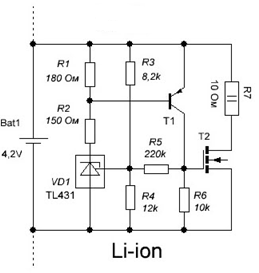
\includegraphics[width=0.4\linewidth]{img/chem_pass_tl431.png}
    \caption{Схема пассивной балансировки на чипе TL-431}
    \label{fig:tl431}
\end{figure}

Данный метод прост в реализации. На каждую ячейку приходится балансировочный резистор 
и небольшая автоматическая обвязка, которая включает балансировку в нужном диапазоне напряжений.
Для примера можно расмотреть схему на базе чипа TL-431. (Рис.\ref{fig:tl431}). (Подробнее в статье \cite{8898267})



\subsection{Активная балансировка}
В методах активной балансировки используются различные накопители энергии.
Алгоритм зарядки перенаправляет энергию от перезаряженной ячейке к менее заряженной.
Основные элементы таких схем это конденсаторы, дроссели, трансформаторы. 
Реже используются импульсные dc-dc преобразователи.

\begin{figure}[h]
    \centering
    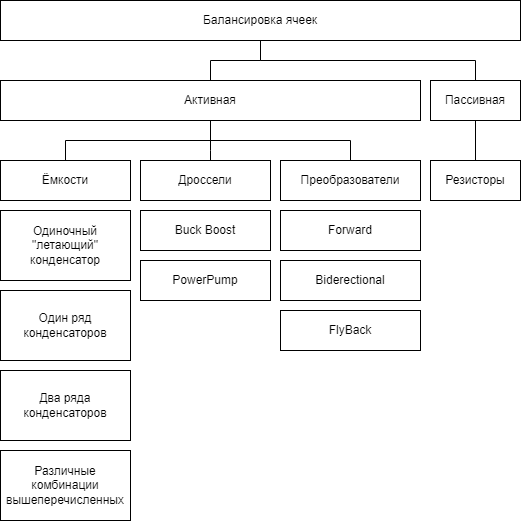
\includegraphics[width=0.6\linewidth]{img/classification.png}
    \caption{Методы балансировки}
    \label{fig:classification}
\end{figure}

\subsubsection{Методы на основе только емкостей}

\subsubsection{Методы на основе только дросселей}

\subsubsection{Метод на основе DC-DC преобразователей}

\subsubsection{Другие методы}

\subsection{Балансировка \glqq без потерь\grqq}
\input{notes/rewiew/noloss_balacing.tex}

\section{Способы организации (модульность BMS)}
\textbf{Монолитная BMS ---} разработаны для определенных конфигураций блоков. Они предлагают простоту и экономичность. 
Немодульные решения BMS предполагается использовать там, где размер и конфигурация аккумуляторной батареи остаются постоянными. 
Они устраняют необходимость в дополнительной проводке и обеспечивают простое решение. 
Не модульная система часто задрудняет обслуживание батареи, в частности замена отдельных неисправных ячеек.

\textbf{Модульная система управления ---} состоит из нескольких блоков, которые можно легко соединять или отключать для реализации различных конфигураций батарей. 
Это обеспечивает гибкость при создании батареи, масштабируемость, простоту обслуживания.
Однако модульные решения BMS могут иметь большее кол-во проводки и усложнение элементов корпуса, что может отразится на цене и весе батареи.

Примером модульной системы является проект с отрытым исходным кодом --- Smart BMS (см. \figurename\ref{fig:smart_bms})
\begin{figure}[h]
	\centering
	\begin{minipage}{0.45\linewidth}
		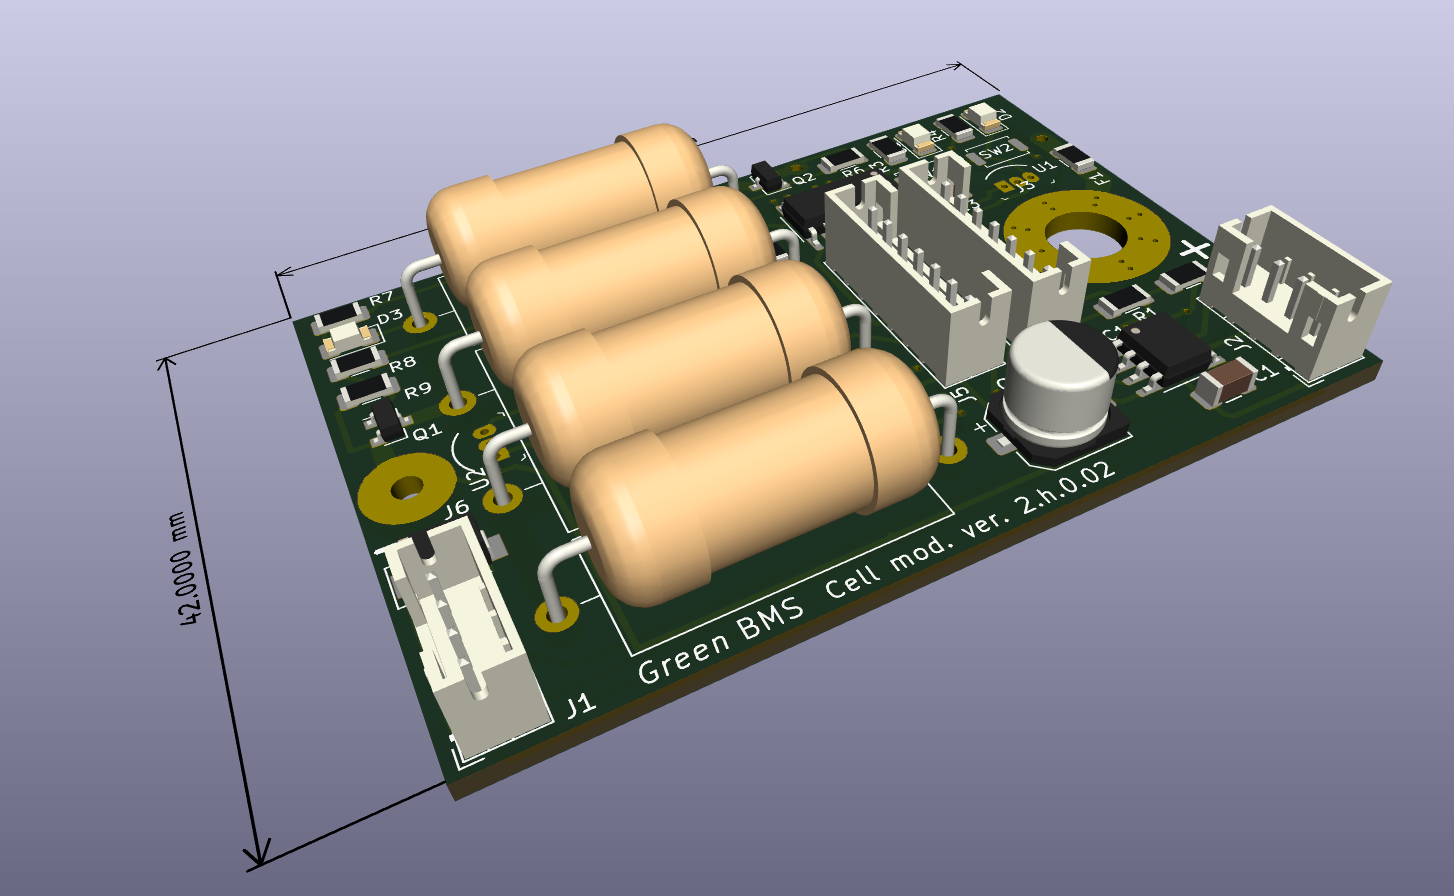
\includegraphics[width=\linewidth]{img/smart_bms_cell_1.png}
		\subcaption{Плата-slave(вид сбоку)}
		% \label{fig:smart_bms_slave_1}
	\end{minipage}
	\begin{minipage}{0.45\linewidth}
	    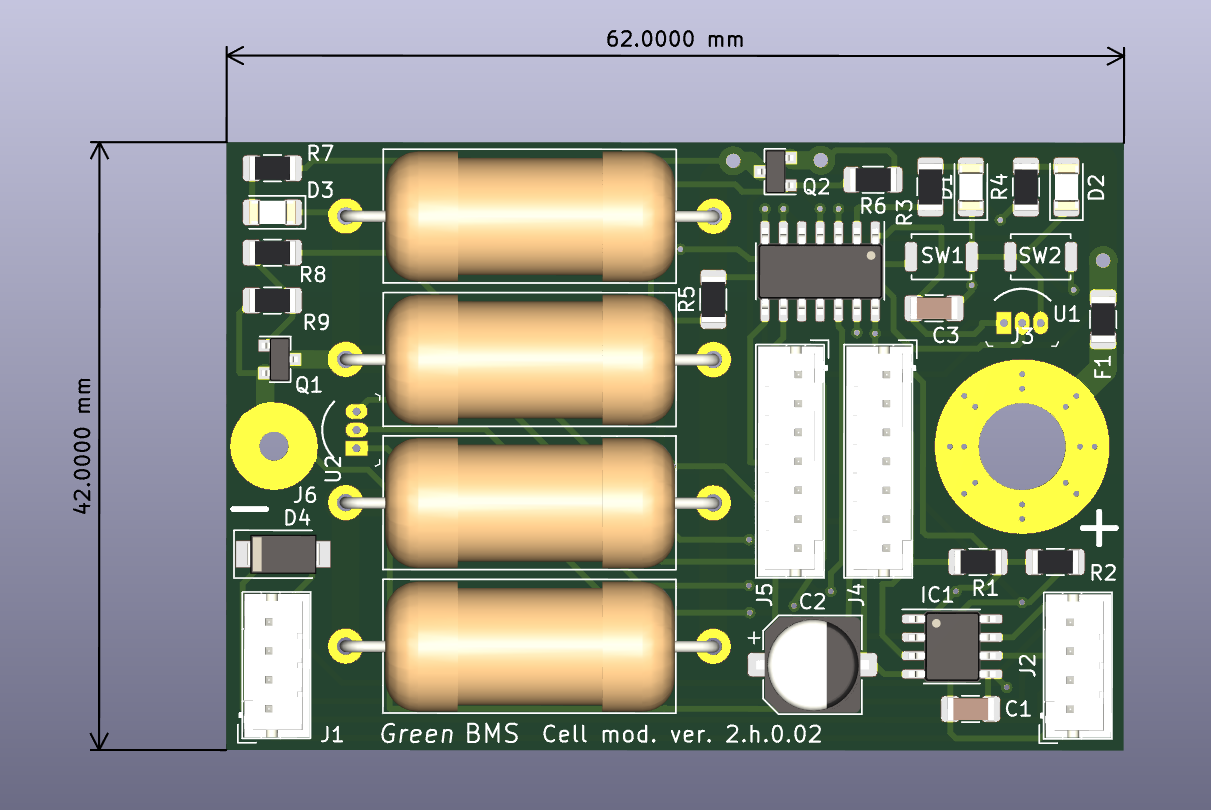
\includegraphics[width=\linewidth]{img/smart_bms_cell_2.png}
	    \subcaption{Плата-slave(вид сверху)}
	    % \label{fig:smart_bms_slave_2}
        \end{minipage} \\	
	\begin{minipage}{0.45\linewidth}
	    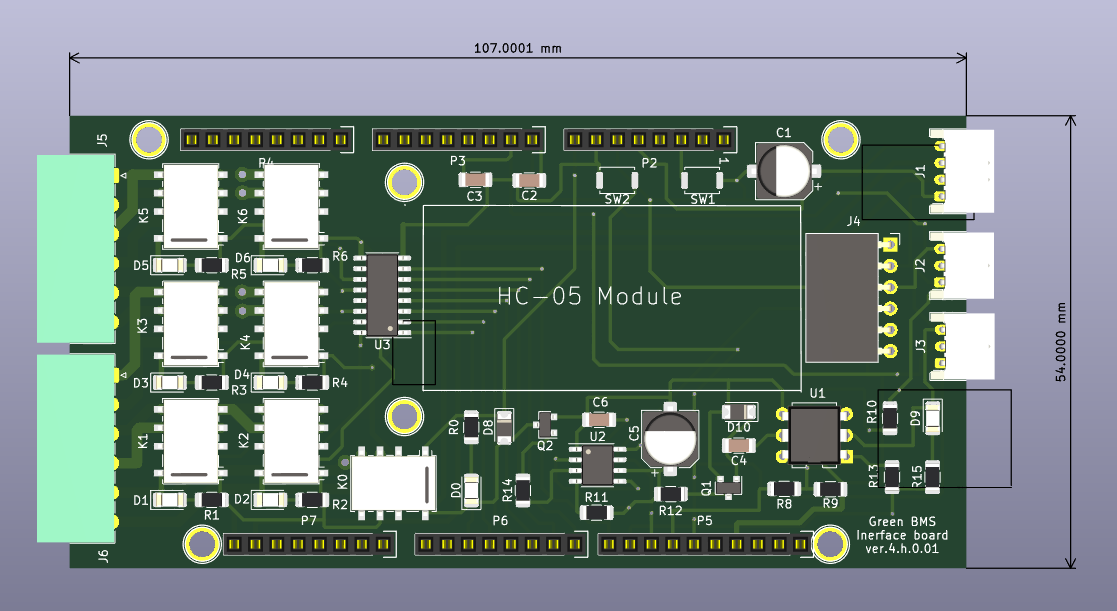
\includegraphics[width=\linewidth]{img/smart_bms_ctrl.png}
	    \subcaption{Плата-мастер}
	    % \label{fig:smart_bms_master}
    \end{minipage}
\caption{Составляющие Smart BMS}
\label{fig:smart_bms}
\end{figure}

\section{Решения сущевствующие на рынке}
\subsection{Tesla}
При анализе технических решений целесообразно уделить внимание разработкам компаний, 
которые занимают лидирующие позиции в данной области. Одной из таких компаний является "Tesla Inc". 
Далее будет приведено устройство батареи, широко известной модели "Tesla Model S".



\begin{figure}[h]
    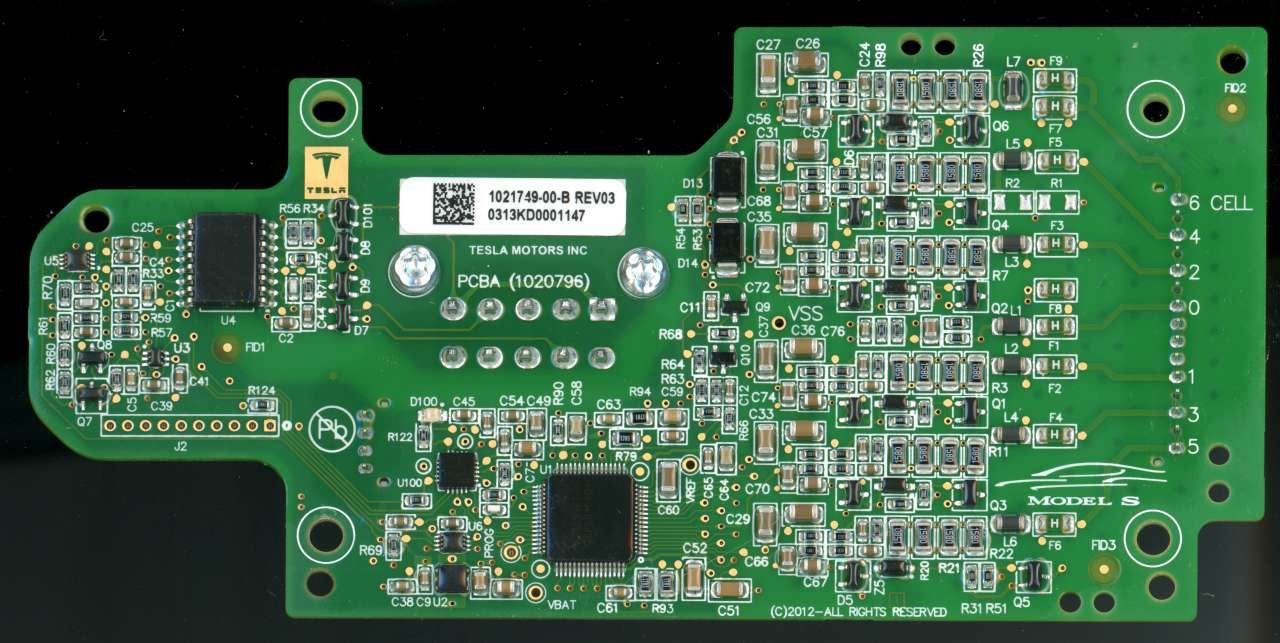
\includegraphics[width=\linewidth]{img/tesla_bms.jpg}
    \caption{BMS модуля батареи Tesla S}
    \label{fig:tesla_bms}
\end{figure}
% Figure \ref{fig:boat1} shows a boat.

% \begin{figure}[h]
% 	\centering
% 	\begin{minipage}{0.45\linewidth}
% 		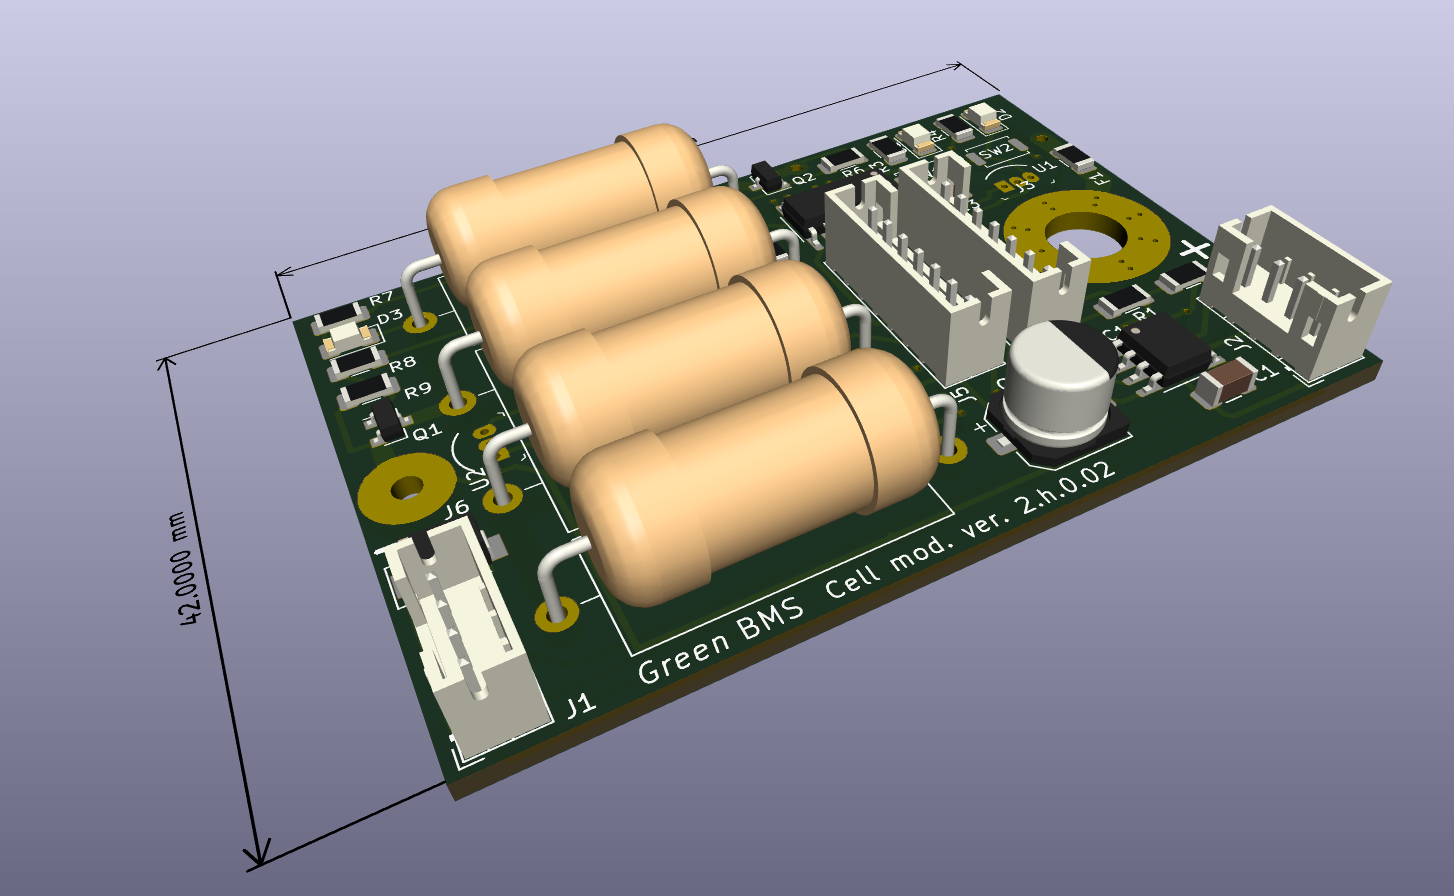
\includegraphics[width=\linewidth]{img/smart_bms_cell_1.png}
% 		\subcaption{Плата-slave(вид сбоку)}
% 		% \label{fig:smart_bms_slave_1}
% 	\end{minipage}
% 	\begin{minipage}{0.45\linewidth}
% 	    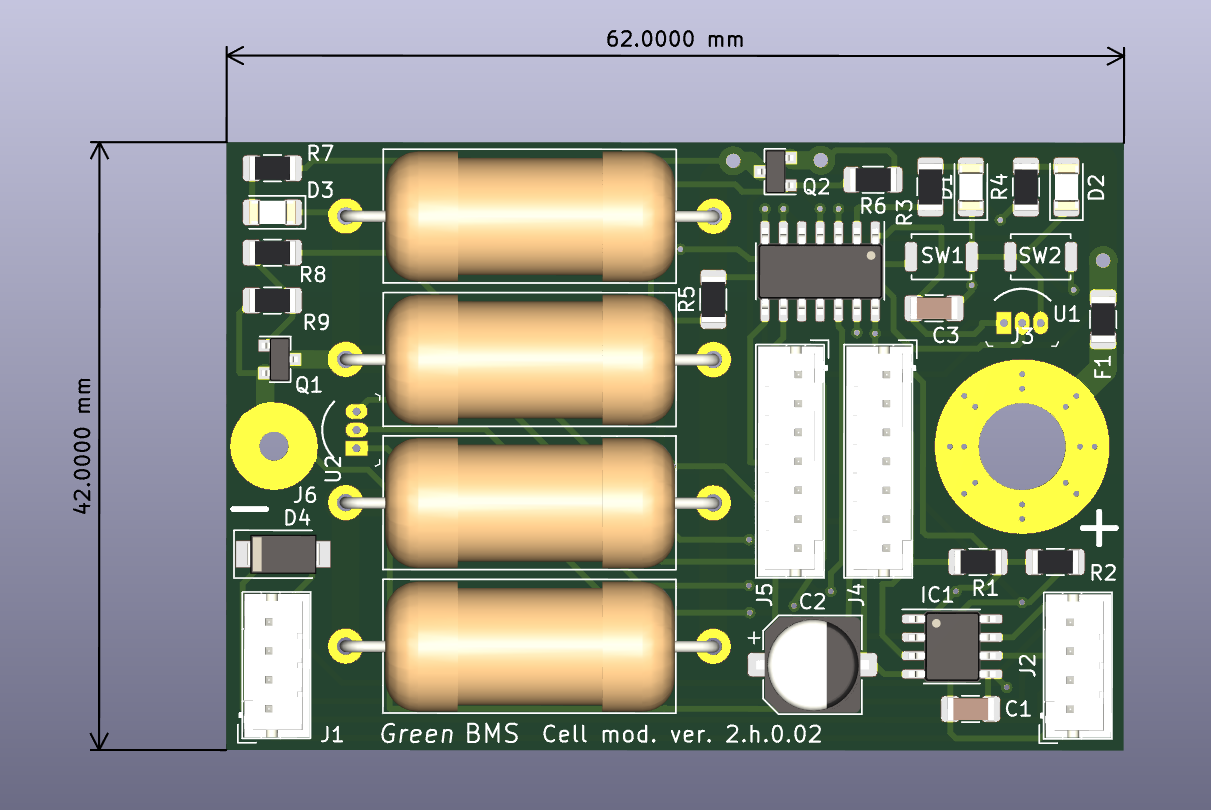
\includegraphics[width=\linewidth]{img/smart_bms_cell_2.png}
% 	    \subcaption{Плата-slave(вид сверху)}
% 	    % \label{fig:smart_bms_slave_2}
%         \end{minipage} \\	
% 	\begin{minipage}{0.45\linewidth}
% 	    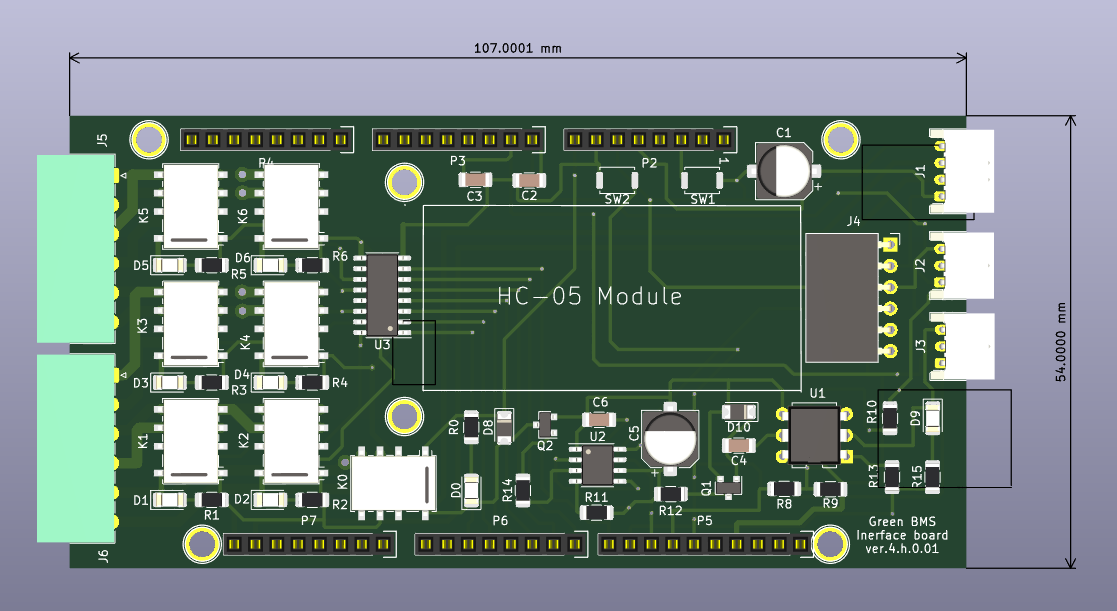
\includegraphics[width=\linewidth]{img/smart_bms_ctrl.png}
% 	    \subcaption{Плата-мастер}
% 	    % \label{fig:smart_bms_master}
%     \end{minipage}
% \caption{Составляющие Smart BMS}
% \label{fig:smart_bms}
% \end{figure}

\subsection{FinDreams Group. Дочернее подразделение BYD}
\input{notes/solutions/byd_bms.tex}

\subsection{AntBMS}
\begin{figure}[!h]
    \centering
    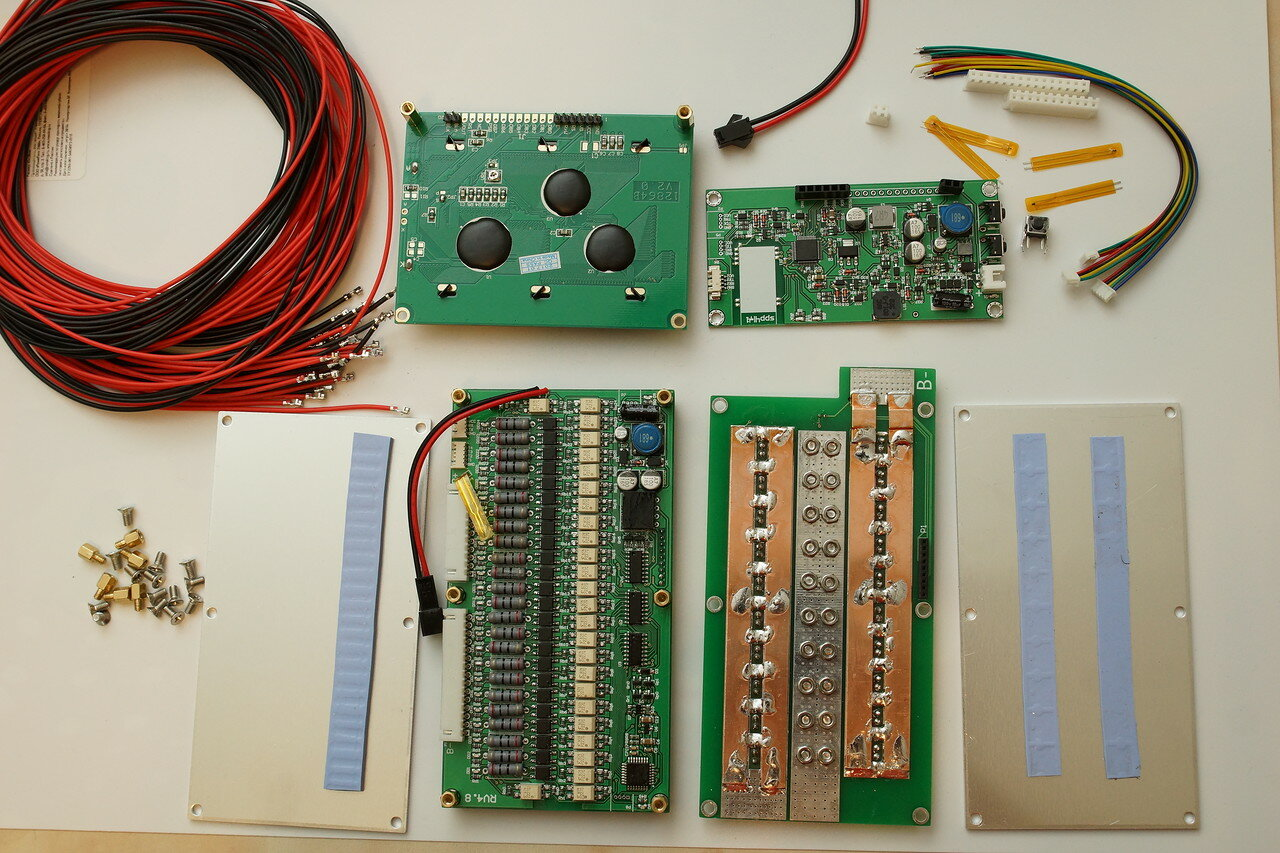
\includegraphics[width=0.9\linewidth]{img/ant_bms.jpg}
    \caption{Модуль пассивной балансировки от компании AntBMS}
    \label{fig:antbms}
\end{figure}

\section{Формализация задачи}

\section{Установка ограничений}

В рамках данной работы предполагается использование батареи, состоящей из ячеек модели
INR-21700-P42A (\hyperref[app:INR21700]{Приложение A}) \\
Конфигурация батареи kSnP -- представляет собой k последовательных блоков, \\
каждый из которых включает n параллельных ячеек (где k составляет порядка 10, а n — от 20 до 30)
Конечная сборка с учетом тока балансировки, рекомендуемого производителем Li-ion батарей, должна иметь балансировочный ток от 0.5n до 1.5n ампер. 
Однако в случае пассивной балансировки ток балансировки будет ограничен мощностью балансировочных резистров.

\section{Сравнение сущевствующих схем}

\section{Поиск оптимальной конфигурации для решения конкретной задачи}
Теперь задача выявить наиболее подходящий метод балансировки.
В статье \cite{daowd2011passive} представлен обзор и сравнение различных способов 
балансировки на основе моделирования в MATLAB Simulink. 
Сравнение проводилось в соответствии с симуляцией балансировки, 
практической реализацией, применением, скоростью балансировки, сложностью, стоимостью, габаритами, 
эффективностью, характерными рабочими токами и напряжениями.



\chapter{Основная часть диплома}
\section{Разработка изделия}
\section{Производство эксперементального изделия}
\section{Испытания эксперементального изделия}
\section{Анализ результатов экспериментов}




\backmatter

\chapter{\bibname}
% \twocolumn
\printbibliography[heading=none]
% \onecolumn

\chapter{Электронные ресурсы}

\chapter{\appendixname}

\appendix

\section{Приложение A: Техническая документация INR-21700-P42A}\label{app:INR21700}
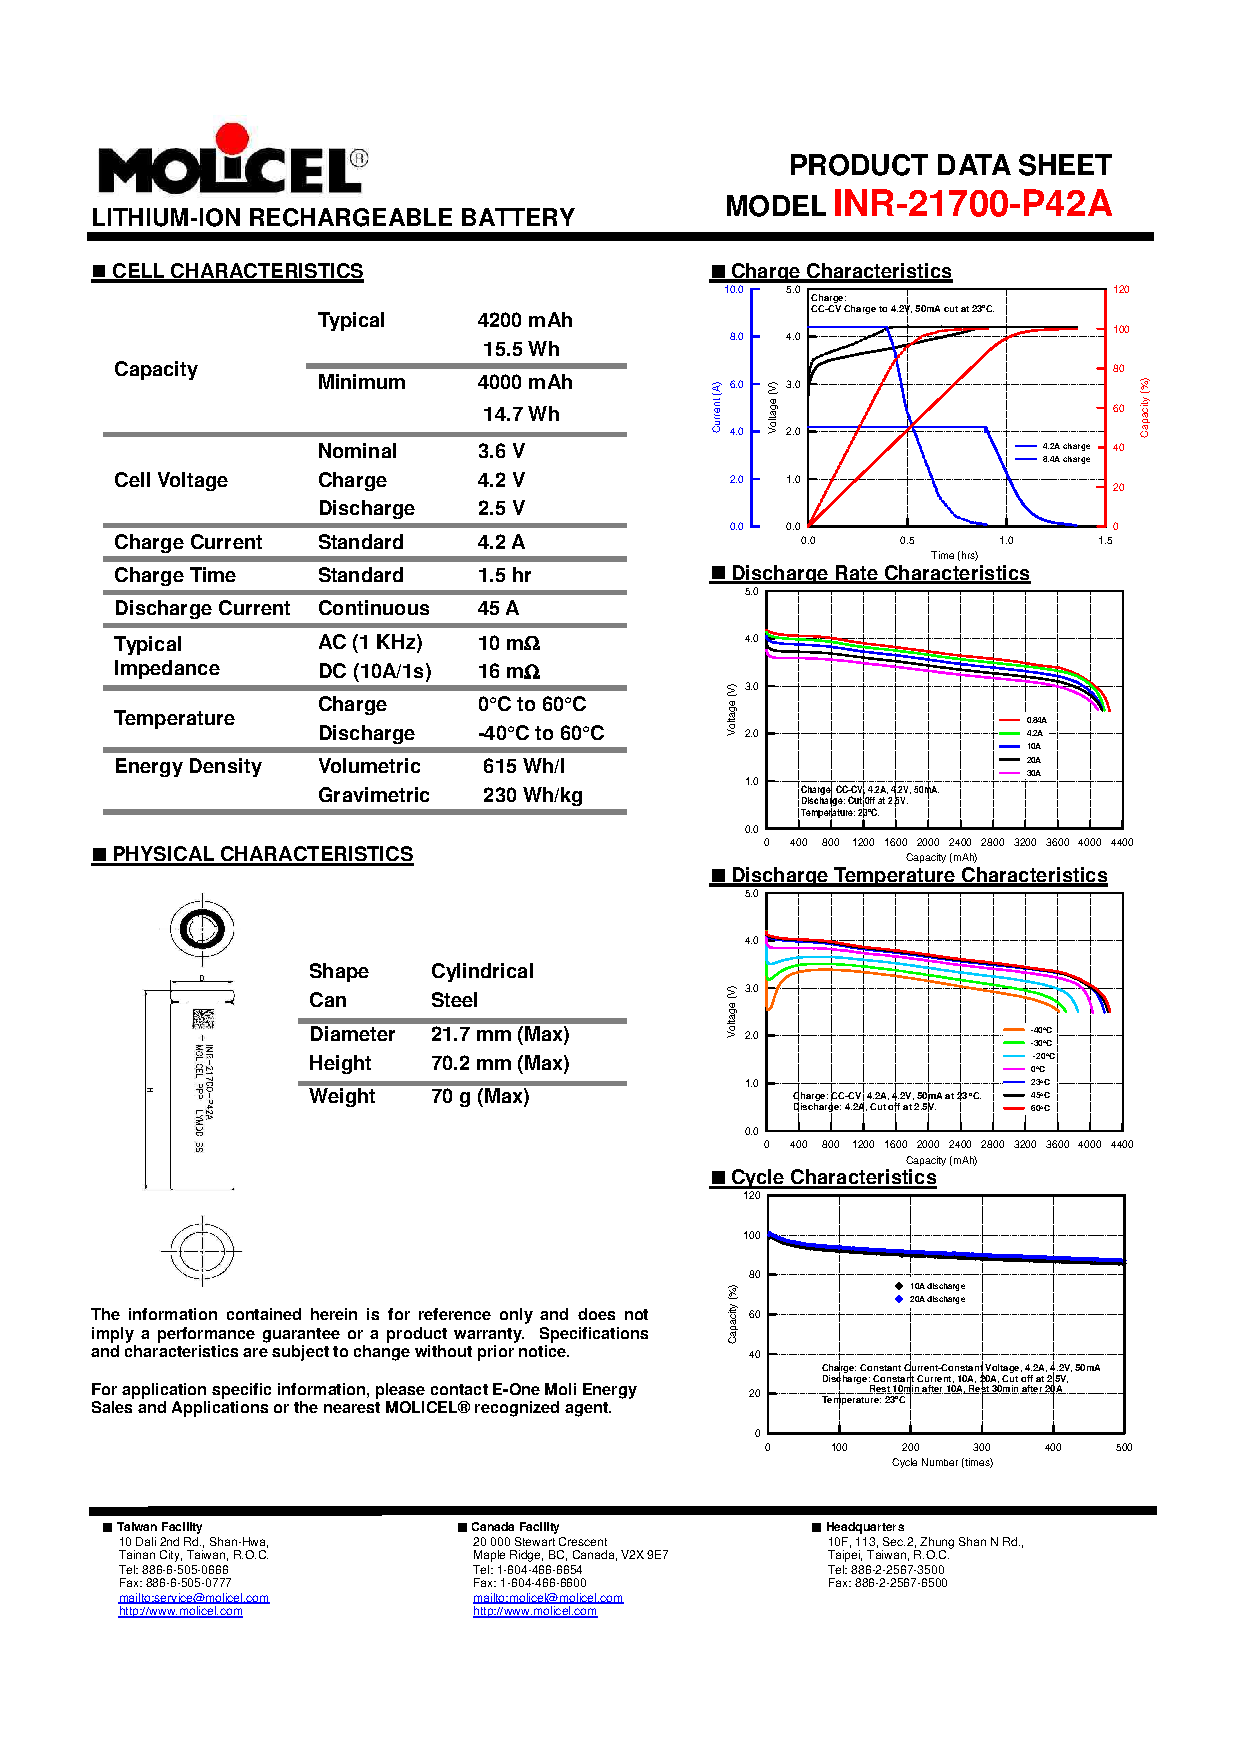
\includepdf[pages=-, scale=0.95]{applications/INR21700P42A-V3-80092.pdf} % Вставляет все страницы PDF





\end{document}
